\documentclass{article}

\title{Dummit \& Foote Ch. 3.5: Transpositions and the Alternating Group}
\author{Scott Donaldson}
\date{Dec. 2023}
\usepackage{amsmath, amsthm, amsfonts, amssymb, enumitem, tabu, tikz}

\begin{document}

\maketitle

\section*{1. (12/6/23)}

In Exercises 1 and 2 of Section 1.3 you were asked to find the cycle decompositions of some permutations. Write each of these permutations as a product of transpositions. Determine which of these is an even permutation and which is an odd permutation.

\vspace{0.5em}
In Exercise 1,
\begin{align*}
    \sigma &= (1, 3, 5)(2, 4) = (1, 3)(1, 5)(2, 4), \text{ odd.} \\
    \tau &= (1, 5)(2, 3), \text{ even.} \\
    \sigma^2 &= (1, 5, 3) = (1, 3)(1, 5), \text{ even.} \\
    \sigma \tau &= (2, 5, 3, 4) = (2, 4)(2, 3)(2, 5), \text{ odd.} \\
    \tau^2 \sigma &= (1, 3, 5)(2, 4) = (1, 5)(1, 3)(2, 4), \text{ odd.}
\end{align*}

In Exercise 2,
\begin{align*}
    \sigma &= (1, 13, 5, 10)(3, 15, 8)(4, 14, 11, 7, 12, 9) \\ &= (1, 10)(1, 5)(1, 13)(3, 8)(3, 15)(4, 9)(4, 12)(4, 7)(4, 11)(4, 14), \text{ even.} \\
    \tau &= (1, 14)(2, 9, 15, 13, 4)(3, 10)(5, 12, 7)(8, 11) \\ &= (1, 14)(2, 4)(2, 13)(2, 15)(2, 9)(3, 10)(5, 7)(5, 12)(8, 11), \text{ odd.} \\
    \sigma^2 &= (1, 5)(3, 8, 15)(4, 11, 12)(7, 9, 4)(10, 13) \\ &= (1, 15)(3, 15)(3, 8)(4, 12)(4, 11)(7, 4)(7, 9)(10, 13), \text{ even.} \\
    \sigma \tau &= (1, 11, 3)(2, 4)(5, 9, 8, 7, 10, 15)(13, 14) \\ &= (1, 3)(1, 11)(2, 4)(5, 15)(5, 10)(5, 7)(5, 8)(5, 9)(13, 14), \text{ odd.} \\
    \tau \sigma &= (1, 4)(2, 9)(3, 13, 12, 15, 11, 5)(8, 10, 14) \\ &= (1, 4)(2, 9)(3, 5)(3, 11)(3, 15)(3, 12)(3, 13)(8, 14)(8, 10), \text{ odd.} \\
    \tau^2 \sigma &= (1, 2, 15, 8, 3, 4, 14, 11, 12, 13, 7, 5, 10) \\ &= (1, 10)(1, 5)(1, 7)(1, 13)(1, 12)(1, 11)(1, 14)(1, 4)(1, 3)(1, 8)(1, 15)(1, 2), \\ & \hspace{1.1em} \text{ even.}
\end{align*}

\section*{2. (12/6/23)}

Prove that $\sigma^2$ is an even permutation for every permutation $\sigma$.

\begin{proof}
    We take as given the homomorphism $\epsilon: S_n \rightarrow \{ \pm 1 \}$ defined in this chapter, which determines the sign of every permutation $\sigma \in S_n$.

    If $\sigma$ is an even permutation, then $\epsilon(\sigma) = 1$. It follows that:
    \begin{equation*}
        \epsilon(\sigma^2) = \epsilon(\sigma)\epsilon(\sigma) = 1 \cdot 1 = 1,
    \end{equation*}
    and so $\sigma^2$ is an even permutation.

    If $\sigma$ is an odd permutation, then $\epsilon(\sigma) = -1$. It follows that:
    \begin{equation*}
        \epsilon(\sigma^2) = \epsilon(\sigma)\epsilon(\sigma) = -1 \cdot -1 = 1,
    \end{equation*}
    and so $\sigma^2$ is an even permutation.

    Since for every $\sigma \in S_n$, $\sigma$ is either an even or an odd permutation, this proves that $\sigma^2$ is an even permutation for every permutation $\sigma$.
\end{proof}

\section*{3. (12/6/23)}

Prove that $S_n$ is generated by $\{ (i, i + 1) \mid 1 \leq i \leq n - 1 \}$.

\begin{proof}
    Since any element of $S_n$ may be written as a product of transpositions, it suffices to show that the set $\{ (i, i + 1) \mid 1 \leq i \leq n - 1 \}$ can generate any transposition. Writing an arbitrary transposition in $S_n$ as $(i, i + a)$, we will prove this by strong induction on $a$ (where $1 \leq a \leq n - i$).

    The base case $a = 1$ is given, since $(i, i + 1)$ is a member of the generating set for all $i \in \{ 1, ..., n - 1 \}$.

    Next, suppose that for all $i \in \{ 1, ..., n - 1\}$ and $a \in \{ 1, ..., n - i \}$, the transposition $(i, i + a - 1)$ can be obtained from the generating set. So we have the transpositions $(i + a - 1, i + a)$ (in the generating set) and $(i, i + a - 1)$ (from the inductive hypothesis). Then:
    \begin{equation*}
        (i + a - 1, i + a)(i, i + a - 1)(i + a - 1, i + a) = (i, i + a),
    \end{equation*}
    so we can obtain the transposition $(i, i + a)$. This concludes the proof that the set $\{ (i, i + 1) \mid 1 \leq i \leq n - 1 \}$ can generate any transposition, and therefore generates all of $S_n$.
\end{proof}

\section*{4. (12/7/23)}

Show that $S_n = \langle (1, 2), (1, 2, 3, ..., n) \rangle$ for all $n \geq 2$.

\begin{proof}
    Note that:
    \begin{align*}
        & \hspace{1.3em} (1, 2, 3, ..., n)(1, 2)(1, 2, 3, ..., n)^{-1} \\
        &= (1, 2, 3, ..., n)(1, 2)(1, n, n - 1, ..., 2) \\
        &= (2, 3),
    \end{align*}
    and in general,
    \begin{align*}
        & \hspace{1.3em} (1, 2, 3, ..., n)(i, i + 1)(1, 2, 3, ..., n)^{-1} \\
        &= (1, 2, 3, ..., n)(i, i + 1)(1, n, n - 1, ..., 2) \\
        &= (i + 1, i + 2)
    \end{align*}
    for $1 \leq i \leq n - 1$ (if $i = n - 1$, then the resulting transposition is equal to $(1, n)$).

    This shows that every transposition of adjacent integers can be obtained from $\langle (1, 2), (1, 2, 3, ..., n) \rangle$, and from the results of Exercise 3, it therefore generates all of $S_n$.
\end{proof}

\section*{5. (12/7/23)}

Show that if $p$ is prime, $S_p = \langle \sigma, \tau \rangle$ where $\sigma$ is any transposition and $\tau$ is any $p$-cycle.

\begin{proof}
    Let $\tau = (a_1, a_2, ..., a_p)$ and $\sigma = (a_i, a_{i + k})$, where $1 \leq i < p$ and $i < k \leq p - i$. Note that:
    \begin{align*}
        \tau \sigma \tau^{-1} &= (a_1, a_2, ..., a_p)(a_i, a_{i + k}) \\
        & \hspace{2.5em} (a_1, a_p, a_{p - 1}, ..., a_2) \\
        &= (a_{i + 1}, a_{i + k + 1}), \text{ and so:} \\
        (\tau^2) \sigma (\tau^2)^{-1} = \tau (\tau \sigma \tau^{-1}) \tau^{-1} &= (a_1, a_2, ..., a_p)(a_{i + 1}, a_{i + k + 1}) \\
        & \hspace{2.5em} (a_1, a_p, a_{p - 1}, ..., a_2) \\
        &= (a_{i + 2}, a_{i + k + 2}), \text{ and in general:} \\
        (\tau^n) \sigma (\tau^n)^{-1} = \tau ((\tau^{n - 1}) \sigma (\tau^{n - 1})^{-1}) \tau^{-1} &= (a_1, a_2, ..., a_p)(a_{i + n - 1}, a_{i + k + n - 1}) \\
        & \hspace{2.5em} (a_1, a_p, a_{p - 1}, ..., a_2) \\
        &= (a_{i + n}, a_{i + k + n}),
    \end{align*}
    where all subscripts are taken mod $p$ if they are greater than $p$.


    Next, we define a set:
    \begin{align*}
        \Sigma &= \{ (\tau^n)\sigma(\tau^n)^{-1} \mid 0 \leq n < p \} \\
        &= \{ (a_j, a_{j + k}) \mid 1 \leq j \leq p \}.
    \end{align*}
    Clearly $\Sigma$ is generated by $\sigma$ and $\tau$. We claim that $\Sigma$ generates any transposition of the form $(a_j, a_{j + nk})$, where $1 \leq j \leq p$, $n \geq 1$. We will show this by strong induction on $n$.

    The base case $n = 1$ is given by the construction of $\Sigma$, since it contains all transpositions of the form $(a_j, a_{j + k})$.

    Next, suppose that $\Sigma$ can generate any transposition of the form $(a_j, a_{j + mk})$, where $1 \leq m < n$. Then:
    \begin{equation*}
        \underbrace{(a_j, a_{j + (n - 1)k})}_{m = n - 1} \underbrace{(a_{j + (n - 1)k}, a_{j + nk})}_{m = 1}\underbrace{(a_j, a_{j + (n - 1)k})}_{m = n - 1} = (a_j, a_{j + nk}),
    \end{equation*}
    which shows that we can generate any transposition of the form $(a_j, a_{j + nk})$.

    Now since $p$ is prime, for any transposition $(a_j, a_{j + q})$, we can write $q = nk$ mod $p$ for some $n \geq 1$. Therefore $\Sigma$ can generate any transposition in $S_p$, and it therefore generates all of $S_p$.
\end{proof}

\section*{6. (12/7/23)}

Show that $\langle (1, 3), (1, 2, 3, 4) \rangle$ is a proper subgroup of $S_4$. What is the isomorphism type of this subgroup?

\begin{proof}
    First, we will define a map $\varphi: D_8 \rightarrow \langle (1, 3), (1, 2, 3, 4) \rangle$ and show that it is an isomorphism. Since the order of $D_8$ is strictly less than $S_4$, we will conclude that $\langle (1, 3), (1, 2, 3, 4) \rangle$ is a proper subgroup of $S_4$.

    Define $\varphi$ such that $\varphi(s) = (1, 3)$ and $\varphi(r) = (1, 2, 3, 4)$. We will first show that $\varphi$ is a homomorphism. The orders of $s$ and $r$ hold under $\varphi$, since $s^2 = 1$ and $(1, 3)^2 = (1)$, and $r^4 = 1$ and $(1, 2, 3, 4)^4 = (1)$. Also, the relation in $D_8$ that $sr = r^{-1}s$ holds under $\varphi$:
    \begin{equation*}
        \varphi(s)\varphi(r) = (1, 3)(1, 2, 3, 4) = (1, 2)(3, 4) = (1, 4, 3, 2)(1, 3) = \varphi(r)^{-1} \varphi(s).
    \end{equation*}
    Since $\varphi$ is defined on the generators of $D_8$ to the generators $(1, 3)$ and $(1, 2, 3, 4)$, $\varphi$ is surjective.

    We next show that $\langle (1, 3), (1, 2, 3, 4) \rangle$ contains 8 elements. The cyclic group generated by $(1, 2, 3, 4)$ contains 4 elements. Its left and right cosets with $(1, 3)$ are equal to each other, so there are therefore no other elements that can be generated. Since $|\langle (1, 3), (1, 2, 3, 4) \rangle| = |D_8|$ and there exists a surjective homomorphism between them, $\varphi$ is necessarily an isomorphism, so $\langle (1, 3), (1, 2, 3, 4) \rangle \cong D_8$. We conclude that it is a proper subgroup of $S_4$.
\end{proof}

\section*{8. (12/8/23)}

Prove the lattice of subgroups of $A_4$ given in this text is correct.

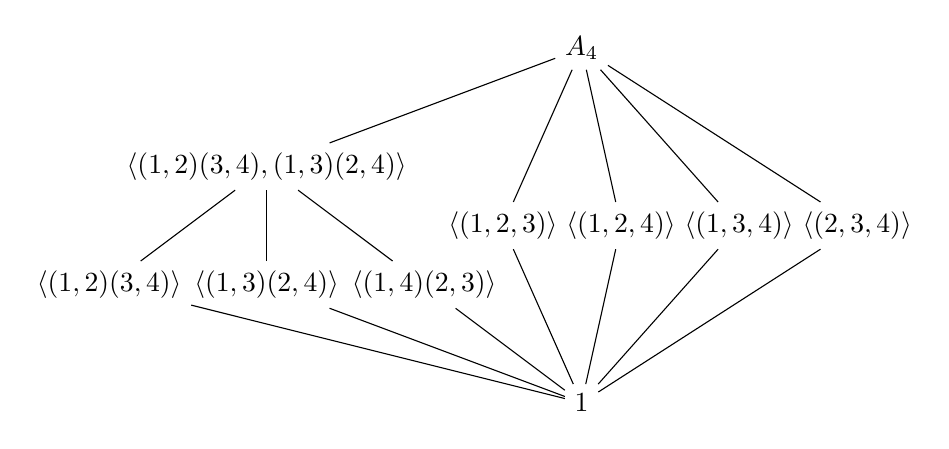
\begin{tikzpicture}[x=2cm,y=1.5cm]
    \node at (0,0)          (1)  {$1$};
    \node at (-3, 1)      (12_34)  {$\langle (1, 2)(3, 4)\rangle$};
    \node at (-2, 1)      (13_24)  {$\langle (1, 3)(2, 4) \rangle$};
    \node at (-1, 1)      (14_23)  {$\langle (1, 4)(2, 3) \rangle$};
    \node at (-2, 2)      (12_34_13_24) {$\langle (1, 2)(3, 4), (1, 3)(2, 4) \rangle$};
    \node at (-0.5, 1.5)   (123) {$\langle (1, 2, 3) \rangle$};
    \node at (0.25, 1.5)   (124) {$\langle (1, 2, 4) \rangle$};
    \node at (1, 1.5)   (134) {$\langle (1, 3, 4) \rangle$};
    \node at (1.75, 1.5)   (234) {$\langle (2, 3, 4) \rangle$};
    \node at (0, 3)       (A4)  {$A_4$};
    
    \draw (1) -- (12_34);
    \draw (1) -- (13_24);
    \draw (1) -- (14_23);
    \draw (1) -- (123);
    \draw (1) -- (124);
    \draw (1) -- (134);
    \draw (1) -- (234);
    \draw (12_34) -- (12_34_13_24);
    \draw (13_24) -- (12_34_13_24);
    \draw (14_23) -- (12_34_13_24);
    \draw (123) -- (A4);
    \draw (124) -- (A4);
    \draw (134) -- (A4);
    \draw (234) -- (A4);
    \draw (12_34_13_24) -- (A4);
\end{tikzpicture}

\begin{proof}
    The alternating group $A_4$ has order $|S_4|/2 = 12$. By Lagrange's Theorem, its proper subgroups must have order 2, 3, 4, or 6.

    It contains no subgroups generated by a single transposition, e.g. $\langle (1, 2) \rangle$, since these contain odd permutations. The other subgroups generated by an element of order 2 are all shown above.

    The lattice also contains all subgroups generated by a single 3-cycle, e.g. $\langle (1, 2, 3) \rangle$. There might be a proper subgroup of order 6 containing one of these. However, as we will show in Exercises 14 and 15, the join of $\langle (1, 2, 3) \rangle$ with another 3-cycle or with a pair of disjoint transpositions produces all of $A_4$. Since there are no other permutations in $A_4$, this implies that there is no proper subgroup containing the cyclic group generated by a 3-cycle.

    Finally, the join of two order 2 subgroups produces $\langle (1, 2)(3, 4), (1, 3)(2, 4) \rangle$. Since this subgroup is of index 3 in $A_4$, there are no other subgroups of $A_4$, and thus the lattice displayed above is correct and complete.
\end{proof}

\section*{9. (12/8/23)}

Prove that the (unique) subgroup of order 4 in $A_4$ is normal and is isomorphic to $V_4$.

\begin{proof}
    From above, the subgroup $\langle (1, 2)(3, 4), (1, 3)(2, 4) \rangle$ is the only subgroup of order 4 in $A_4$. Its generators are both elements of order 2. Since the cyclic group $Z_4$ contains only one element of order 2, it is not isomorphic to $Z_4$. There are only two groups of order 4 up to isomorphism, and therefore it is isomorphic to $V_4$.

    Next, it is normal in $A_4$. We consider the conjugate of its generators by (without loss of generality) the permutation $(1, 2, 3)$:
    \begin{align*}
        (1, 2, 3)(1, 2)(3, 4)(1, 3, 2) &= (1, 4)(2, 3), \text{ and} \\
        (1, 2, 3)(1, 3)(2, 4)(1, 3, 2) &= (1, 2)(3, 4),
    \end{align*}
    both of which lie in $\langle (1, 2)(3, 4), (1, 3)(2, 4) \rangle$. Thus $\langle (1, 2)(3, 4), (1, 3)(2, 4) \rangle$ is normal in $A_4$.
\end{proof}

\section*{10. (12/8/23)}

Find a composition series for $A_4$. Deduce that $A_4$ is solvable.

\begin{proof}[Solution]
    \begin{equation*}
        1 \leq \langle (1, 2)(3, 4) \rangle \leq \langle (1, 2)(3, 4), (1, 3)(2, 4) \rangle \leq A_4
    \end{equation*}
    is a composition series for $A_4$. The lower two quotient groups are isomorphic to $Z_2$, a simple group, and $|A_4:\langle (1, 2)(3, 4), (1, 3)(2, 4) \rangle| = 3$, which implies that the last quotient group is isomorphic to $Z_3$, also simple. Since these quotient groups are also abelian, this implies that $A_4$ is solvable.
\end{proof}

\section*{11. (12/12/23)}

Prove that $S_4$ has no subgroup isomorphic to $Q_8$.

\begin{proof}
    Suppose that $A \leq S_4$ and that $\varphi: Q_8 \rightarrow A$ is an isomorphism. In $Q_8$, $|i| = 4$, so $\varphi$ must assign $i$ to a permutation whose cycle decomposition is a 4-cycle. Without loss of generality, suppose that $\varphi(i) = (1, 2, 3, 4)$. 
    
    
    Because $\varphi$ is injective, we cannot have $\varphi(j) = (1, 2, 3, 4)$. Also, $(1, 4, 3, 2) = (1, 2, 3, 4)^{-1}$, and since $j \neq -i$, we cannot have $\varphi(j) = (1, 4, 3, 2)$, so $\varphi(j)$ must equal some other 4-cycle in $S_4$. The remaining options are:
    \begin{align*}
        \varphi(j) = (1, 2, 4, 3), (1, 3, 2, 4), (1, 3, 4, 2), \text{ or } (1, 4, 2, 3).
    \end{align*}
    Note that, in $Q_8$, $i^2 = j^2 = -1$. Under $\varphi$, we have $\varphi(i)^2 = (1, 3)(2, 4)$. However, for none of the remaining 4-cycles we might assign $j$ to do we have $\varphi(j)^2 = (1, 3)(2, 4)$. Thus there is no element to which we can assign $j$ and have $\varphi$ be an isomorphism. Therefore there $S_4$ has no subgroup isomorphic to $Q_8$.
\end{proof}

\section*{12. (12/12/23)}

Prove that $A_n$ contains a subgroup isomorphic to $S_{n - 2}$ for each $n \geq 3$.

\begin{proof}
    We define a map $\varphi: S_{n - 2} \rightarrow A_n$ by:
    \begin{equation*}
        \varphi(\sigma) =
        \begin{cases}
            \sigma      & \text{if $\sigma$ is even} \\
            \sigma \cdot (n - 1, n)  & \text{if $\sigma$ is odd}
        \end{cases}.
    \end{equation*}
    Now noting that $\frac{1}{2}n(n - 1) > 1$ for all $n \leq 3$, we conclude that:
    \begin{align*}
        \frac{1}{2}n(n - 1) & > 1 \\
        \frac{1}{2}n(n - 1)(n - 2) \cdot ... \cdot 2 \cdot 1 & > (n - 2) \cdot ... \cdot 2 \cdot 1 \\
        \frac{1}{2}(n!) & > (n - 2)! \\
        |A_n| & > S_{n - 2}.
    \end{align*}
    Since the order of $A_n$ is strictly greater than that of $S_{n - 2}$, $\varphi$ cannot be surjective. It is trivial to show that it is injective, and so if $\varphi$ is a homomorphism, then its image is a proper subgroup of $A_n$ isomorphic to $S_{n - 2}$.

    Let $\sigma_1, \sigma_2 \in S_{n - 2}$ and consider the different cases:
    \begin{itemize}[itemsep=0em]
        \item Both even permutations. Then $\sigma_1 \sigma_2$ is even, so:
              \begin{equation*}
                \varphi(\sigma_1 \sigma_2) = \sigma_1 \sigma_2 = \varphi(\sigma_1) \varphi(\sigma_2)
              \end{equation*}
        \item Both odd permutations. Then $\sigma_1 \sigma_2$ is even. Note that each $\sigma \in S_{n - 2}$ is disjoint with the transposition $(n - 1, n)$, and so commutes with it in $A_n$. Therefore:
              \begin{align*}
                  \varphi(\sigma_1) \varphi(\sigma_2) &= \sigma_1 \cdot (n - 1, n) \cdot \sigma_2 \cdot (n - 1, n) \\ &= \sigma_1 \sigma_2 (n - 1, n)(n - 1, n) \\
                  &= \sigma_1 \sigma_2, \text{ and} \\
                  \varphi(\sigma_1 \sigma_2) &= \sigma_1 \sigma_2.
              \end{align*}
        \item One even, one odd. Let $\sigma_1$ be an even permutation and $\sigma_2$ be odd (and their product is odd). Then:
              \begin{align*}
                \varphi(\sigma_1 \sigma_2) &= \sigma_1 \sigma_2 \cdot (n - 1, n), \text{ and} \\
                \varphi(\sigma_1) \varphi(\sigma_2) &= \sigma_1 \sigma_2 \cdot (n - 1, n).
              \end{align*}
    \end{itemize}
    This proves that $\varphi$ is a homomorphism, and since it is injective but not surjective, its image is a subgroup of $A_n$ that is isomorphic to $S_{n - 2}$.
\end{proof}

\section*{13. (12/13/23)}

Prove that every element of order 2 in $A_n$ is the square of an element of order 4 in $S_n$. [An element of order 2 in $A_n$ is a product of $2k$ commuting transpositions.]

\begin{proof}
    From Chapter 1.3, Exercise 15, the order of a permutation is equal to the least common multiple of the lengths of cycles in its cycle decomposition. Therefore an element of order 2 in $A_n \leq S_n$ must have a cycle decomposition with only 2-cycles, that is, it must be the product of disjoint transpositions.

    Let $\sigma \in A_n$ have order 2 with the cycle decomposition:
    \begin{equation*}
        (a_1, b_1)(c_1, d_1)...(a_k, b_k)(c_k, d_k).
    \end{equation*}
    Then $\sigma$ is the square of the permutation in $S_n$ with the cycle decomposition:
    \begin{equation*}
        (a_1, c_1, b_1, d_1)...(a_k, c_k, b_k, d_k).
    \end{equation*}
    Since all of these cycles are disjoint, the permutation has order 4, so every element of order 2 in $A_n$ is the square of an element of order 4 in $S_n$.
\end{proof}

\section*{14. (12/13/23)}

Prove that the subgroup of $A_4$ generated by any element of order 2 and any element of order 3 is all of $A_4$.

\begin{proof}
    Without loss of generality, we consider the subgroups generated by an arbitrary element of order 3 and $(1, 2)(3, 4) \in A_4$. We claim that the product of $(1, 2)(3, 4)$ and $\sigma$, a 3-cycle is always another 3-cycle that is not the inverse of $\sigma$:
    \begin{align*}
        (1, 2)(3, 4) \cdot (1, 2, 3) &= (2, 4, 3) \\
        (1, 2)(3, 4) \cdot (1, 2, 4) &= (2, 3, 4) \\
        (1, 2)(3, 4) \cdot (1, 3, 4) &= (1, 4, 2) \\
        (1, 2)(3, 4) \cdot (2, 3, 4) &= (1, 2, 4).
    \end{align*}
    For each of the four 3-cycles on the right-hand side of the equation, multiplying them on the left by $(1, 2)(3, 4)$ produces the 3-cycle on the left-hand side of the equation.

    Now the generated subgroup contains the the identity, $(1, 2)(3, 4)$, and two distinct 3-cycles (as well as their inverses), for a total of 6 elements. From the table above, left-multiplying one of the inverses of the 3-cycles by $(1, 2)(3, 4)$ produces yet another 3-cycle, so the subgroup contains at least 7 elements. By Lagrange's Theorem, its order must divide $|A_4| = 12$. Therefore, its order must be 12, that is, all of $A_4$.
\end{proof}

\end{document}